%Dave's handout 6.2 Definite Integrals and Net Change of a Function

\vspace{-0.25 in}
\begin{framed}
\subsection*{Objectives}
\begin{itemize}
    \item Understand the procedure for computing the value of a \textbf{definite integral}.
    \item Be able to use definite integrals to determine the \textbf{net change} in the value of a function.
    \item Be able to use and interpret the net change in the value of a function in application problems. 
\end{itemize}

%%%Reading Assignment%%%
\subsection*{Suggested Reading:}
\begin{itemize}
\item \cite{Calaway}\footnotemark[1]
   \begin{itemize}
        \item \emph{Section 3.2 The Fundamental Theorem and Antidifferentiation}
        \begin{itemize}
            \item \emph{The Fundamental Theorem of Calculus}
        \end{itemize}
    \end{itemize}

\item \cite{openstax}\footnotemark[2]\textsuperscript{,}\footnotemark[3]
    \begin{itemize}
        \item \emph{Section 5.3 The Fundamental Theorem of Calculus}
        \begin{itemize}
            \item \emph{Fundamental Theorem of Calculus, Part 2: The Evaluation Theorem}
        \end{itemize}
        \item \emph{Section 5.4 Integration Formulas and the Net Change Theorem}
        \begin{itemize}
            \item \emph{The Net Change Theorem}
            \item \emph{Applying the Net Change Theorem}
        \end{itemize}
    \end{itemize}
    
\end{itemize}
%\subsection*{Supplemental Materials:}
%%%Key Terms%%%
\subsection*{Key Terms and Concepts:} 

\begin{multicols}{2}
\begin{itemize}
    \item Definite integrals
    \item Limits of integration
    \item Net change in the value of a function
\end{itemize}
\end{multicols}
\end{framed}
\footnotetext[1]{Available free to download from \url{http://www.opentextbookstore.com/details.php?id=14} .}
\footnotetext[2]{Available free to download from \url{https://openstax.org/details/books/calculus-volume-1} .}
\footnotetext[3]{Disregard any examples with trigonometry.}

\newpage
%%%%%%%%%%START LESSON CONTENT%%%%%%%%%%%%%
%\noindent\makebox[\linewidth]{\rule{\textwidth}{0.8pt}}
\Opensolutionfile{ans}[ans21]
\Opensolutionfile{ansL}[ansL21]
%%%%%%%%%%%%%%%%Introduction (OpenStax 5.3 Fundamental Theorem of Calculus and Applied Calculus Chapter 3 Lesson 2%%%%%%%%%%%%%%%%%%%%%%%%%%%%%

\noindent The relationship between differentiation and integration was discovered and explored by both \emph{Sir Isaac Newton and Gottfried Wilhelm Leibniz} (among others) during the late 1600s and early 1700s, and it is codified in what we now call the \textbf{Fundamental Theorem of Calculus}. Its very name indicates how central this theorem is to the entire development of calculus. Calculus is one of the most significant intellectual structures in the history of human thought, and the Fundamental Theorem of Calculus is a most important brick in that beautiful structure. The theorem provides scientists with the necessary tools to explain many phenomena. Using calculus, astronomers could finally determine distances in space and map planetary orbits. Everyday financial problems such as calculating marginal costs or predicting total profit could now be handled with simplicity and accuracy. Engineers could calculate the bending strength of materials or the three-dimensional motion of objects. Our view of the world was forever changed with calculus.\\

\noindent \textbf{The Fundamental Theorem of Calculus} is comprised of two parts. The \emph{Fundamental Theorem of Calculus, Part 1}, establishes the relationship between differentiation and integration. This lesson however does not cover the first part of the Fundamental Theorem of Calculus\footnotemark. In this lesson,  we examine the \textbf{Fundamental Theorem of Calculus, Part 2} which is perhaps the most important theorem in calculus. It gives us powerful and useful techniques for evaluating  \textbf{definite integrals}. \\

\footnotetext{The explanation of the first part of the theorem can be found in section 5.3 from \cite{openstax}}

\begin{tcolorbox}[title = {The Definite Integral and Its Notation}]
Suppose we are given a function $f(x)$ that is continuous over an interval $[a,b]$, and the function $F(x)$ is any antiderivative of $f(x)$ (that is, $F'(x)=f(x)$. The definite integral of $f$ from $a$ to $b$ is written
\begin{equation}
    \int_{a}^{b} f(x) dx
\end{equation}

The numbers $a$ and $b$ are called the \textbf{limits of integration}; $a$ is the \textbf{lower limit}, and $b$ is the \textbf{upper limit}.

\end{tcolorbox}

\begin{tcolorbox}[title = {The Fundamental Theorem of Calculus, Part 2 (also known as the evaluation theorem)}]
\noindent If $f(x)$ is continuous over an interval $[a,b]$, and the function $F(x)$ is any antiderivative of $f(x)$ (that is, $F'(x)=f(x)$, then 
\begin{equation}\label{eq:evaluationTheorem}
\int_{a}^{b} f(x) dx = F(b)-F(a)    
\end{equation}

\noindent We often see the notation $F(x)\big|_{a}^{b}$ to denote the expression $F(b)-F(a)$. We use this vertical bar and associated \textbf{limits of integration} $a$ and $b$ to indicate that we should evaluate the function $F(x)$ at the \textbf{upper limit} $b$, and subtract the value of the function $F(x)$ evaluated at the \textbf{lower limit} $a$.\\

\end{tcolorbox}
\noindent The theorem states that if we can find an \textbf{antiderivative} for the integrand, then we can evaluate the \textbf{definite integral} by evaluating the antiderivative at the endpoints of the interval and subtracting.

%%%%%%%%%%%%%%%%%%%%Example: Dave's handout 6.2%%%%%%%%%%%%%%%%%%%%%%%%
\begin{example}
Let $f(x)=x^2$. 
\renewcommand{\labelenumi}{\textbf{(\alph{enumi})}}
\begin{enumerate}[leftmargin=*]
\item Find \textbf{the} antiderivative of $f(x)$. That is, evaluate \textbf{the indefinite integral}: $\displaystyle \int f(x) dx$. \vspace*{\stretch{0.5}}
\item Evaluate \textbf{the definite integral}: $\displaystyle \int_{1}^{3} f(x) dx$.\vspace*{\stretch{1}}
\end{enumerate}
\noindent \textbf{Look Back:} Notice the similarity and the difference among  \emph{Antiderivative, Indefinite Integral and Definite Integral}. The final answer of the definite integral is a number while the result of the indefinite integral is a function.
    %%short answer
    \begin{sol}
    \onehalfspacing{
    \begin{enumInline1}
    \item $\displaystyle\frac{1}{3}x^3$
    \item $8\displaystyle\frac{2}{3}$
    \end{enumInline1} }
    \end{sol}
    %%solution
    \begin{solL}
    \renewcommand{\labelenumi}{\textbf{(\alph{enumi})}}
    \begin{enumerate}[leftmargin=*]
    \item \hfill 
    \newline 
    $\int x^2\,dx=\dfrac{x^{2+1}}{2+1}+C=\dfrac{x^3}{3}$ \qquad by Power Rule
    \item \hfill 
    \newline 
        \begin{displaymath}
            \begin{split}
            F(x)&=\dfrac{x^3}{3}+C \qquad \text{Antiderivative from part (a)}\\
            F(3)&=\dfrac{3^3}{3}+C=9+C  \qquad \text{Evaluate the antiderivative at the upper limit:}\: x=3\\
            F(1)&=\dfrac{1^3}{3}+C=\frac{1}{3}+C  \qquad \text{Evaluate the antiderivative at the lower limit:}\: x=1\\
            \int^3_1 x^2\,dx&=F(3)-F(1)\qquad \text{The Fundamental Theorem of Calculus}\\
            &=(9+C)-\left(\frac{1}{3}+C\right) \\
            &=9+C-\frac{1}{3}-C\\
            &=\frac{26}{3}=8\frac{2}{3}
            \end{split}
        \end{displaymath}
    \end{enumerate}
    
    \end{solL}
    
\end{example}

\begin{tcolorbox}[title = {Net Change Theorem}]%Calculus I from OpenStax 5.4
Using the definition of a definite integral from the \emph{Fundamental Theorem of Calculus, Part 2}, we can alter the notation in Equation \ref{eq:evaluationTheorem} slightly and re-write the definition as follows (recall that $ F'(x)=f(x)$): 
\begin{equation}\label{eq:netchange1}
\int_{a}^{b} F'(x) dx= F(b)-F(a)
\end{equation}
By adding $F(a)$ from both sides of the equation above yields the equivalent equation, which one we use depends on the application.
\begin{equation}\label{eq:netchange2}
    F(b)=F(a)+\int_{a}^{b} F'(x) dx
\end{equation}
\end{tcolorbox}

\noindent The net change theorem considers the integral of a \emph{rate of change}, that is $F'(x)$ or $f(x)$ above.  The formula can be expressed in two ways. The first in equation \ref{eq:netchange1} is more familiar; it is simply the definite integral defined in equation \ref{eq:evaluationTheorem}. The second formula in equation \ref{eq:netchange2} says that when a quantity changes, the new value equals the initial value plus the integral of the rate of change of that quantity. Net change can be applied to area, distance, and volume, to name only a few applications. Net change accounts for negative quantities automatically without having to write more than
one integral.

%%%%%%%%%%%%%%%%%%%%Example: Dave's handout 6.2%%%%%%%%%%%%%%%%%%%%%%%%
\begin{example}
The value, $V$, of an investment is expected to grow over time.  The expectation is that the rate of increase in value can be approximated  by $V'(t)=1000e^{0.08t}+2000$ dollars per year.  Determine the net increase in the value of the investment over the first 5 years, that is, over the time interval from $t=0$ to $t=5$. 	Round your answer to the nearest dollar.	
    %%short answer
    \begin{sol}
    $V(t)=12500e^{0.08t}+2000t$; $V(t)\big|_0^5\approx 16,148$;  We are expecting the value of the investment to \underline{increase} by approximately \$16,148 over the first 5 years.
    \end{sol}
    %%solution
    \begin{solL}
    ??
    
    \end{solL}
    
\end{example}
\vspace*{\stretch{2}}
\newpage
%%%%%%%%%%%%%%%%%%%%Example: Dave's handout 6.2%%%%%%%%%%%%%%%%%%%%%%%%
\begin{example}
During spring, the bird population, $P$, at a refuge is changing at a rate given by $P'(t)=.8e^{0.04t}-0.2e^{0.0625t}$ hundreds of birds per day.  Let the function $P(t)$ represent the total number of birds at the refuge (in hundreds) at time $t$ days from the first day of spring.Suppose that there were 3,000 birds at the first day of spring.  \\
\newline 
Follow this Desmos link to see the graph of $P'(t)$: \url{https://www.desmos.com/calculator/oofhcxrc5p}\\
Follow this Desmos link to see the graph of $P(t)$: \url{https://www.desmos.com/calculator/zo6auzan1f}
\renewcommand{\labelenumi}{\textbf{(\alph{enumi})}}
\begin{enumerate}[leftmargin=*]
\item Find the formula of $P(x)$.  \vspace*{\stretch{1}}
\item During the first 10 days, what is the net change in total number of birds at the refuge ? 
    \begin{figure}[h!]
        \flushleft
        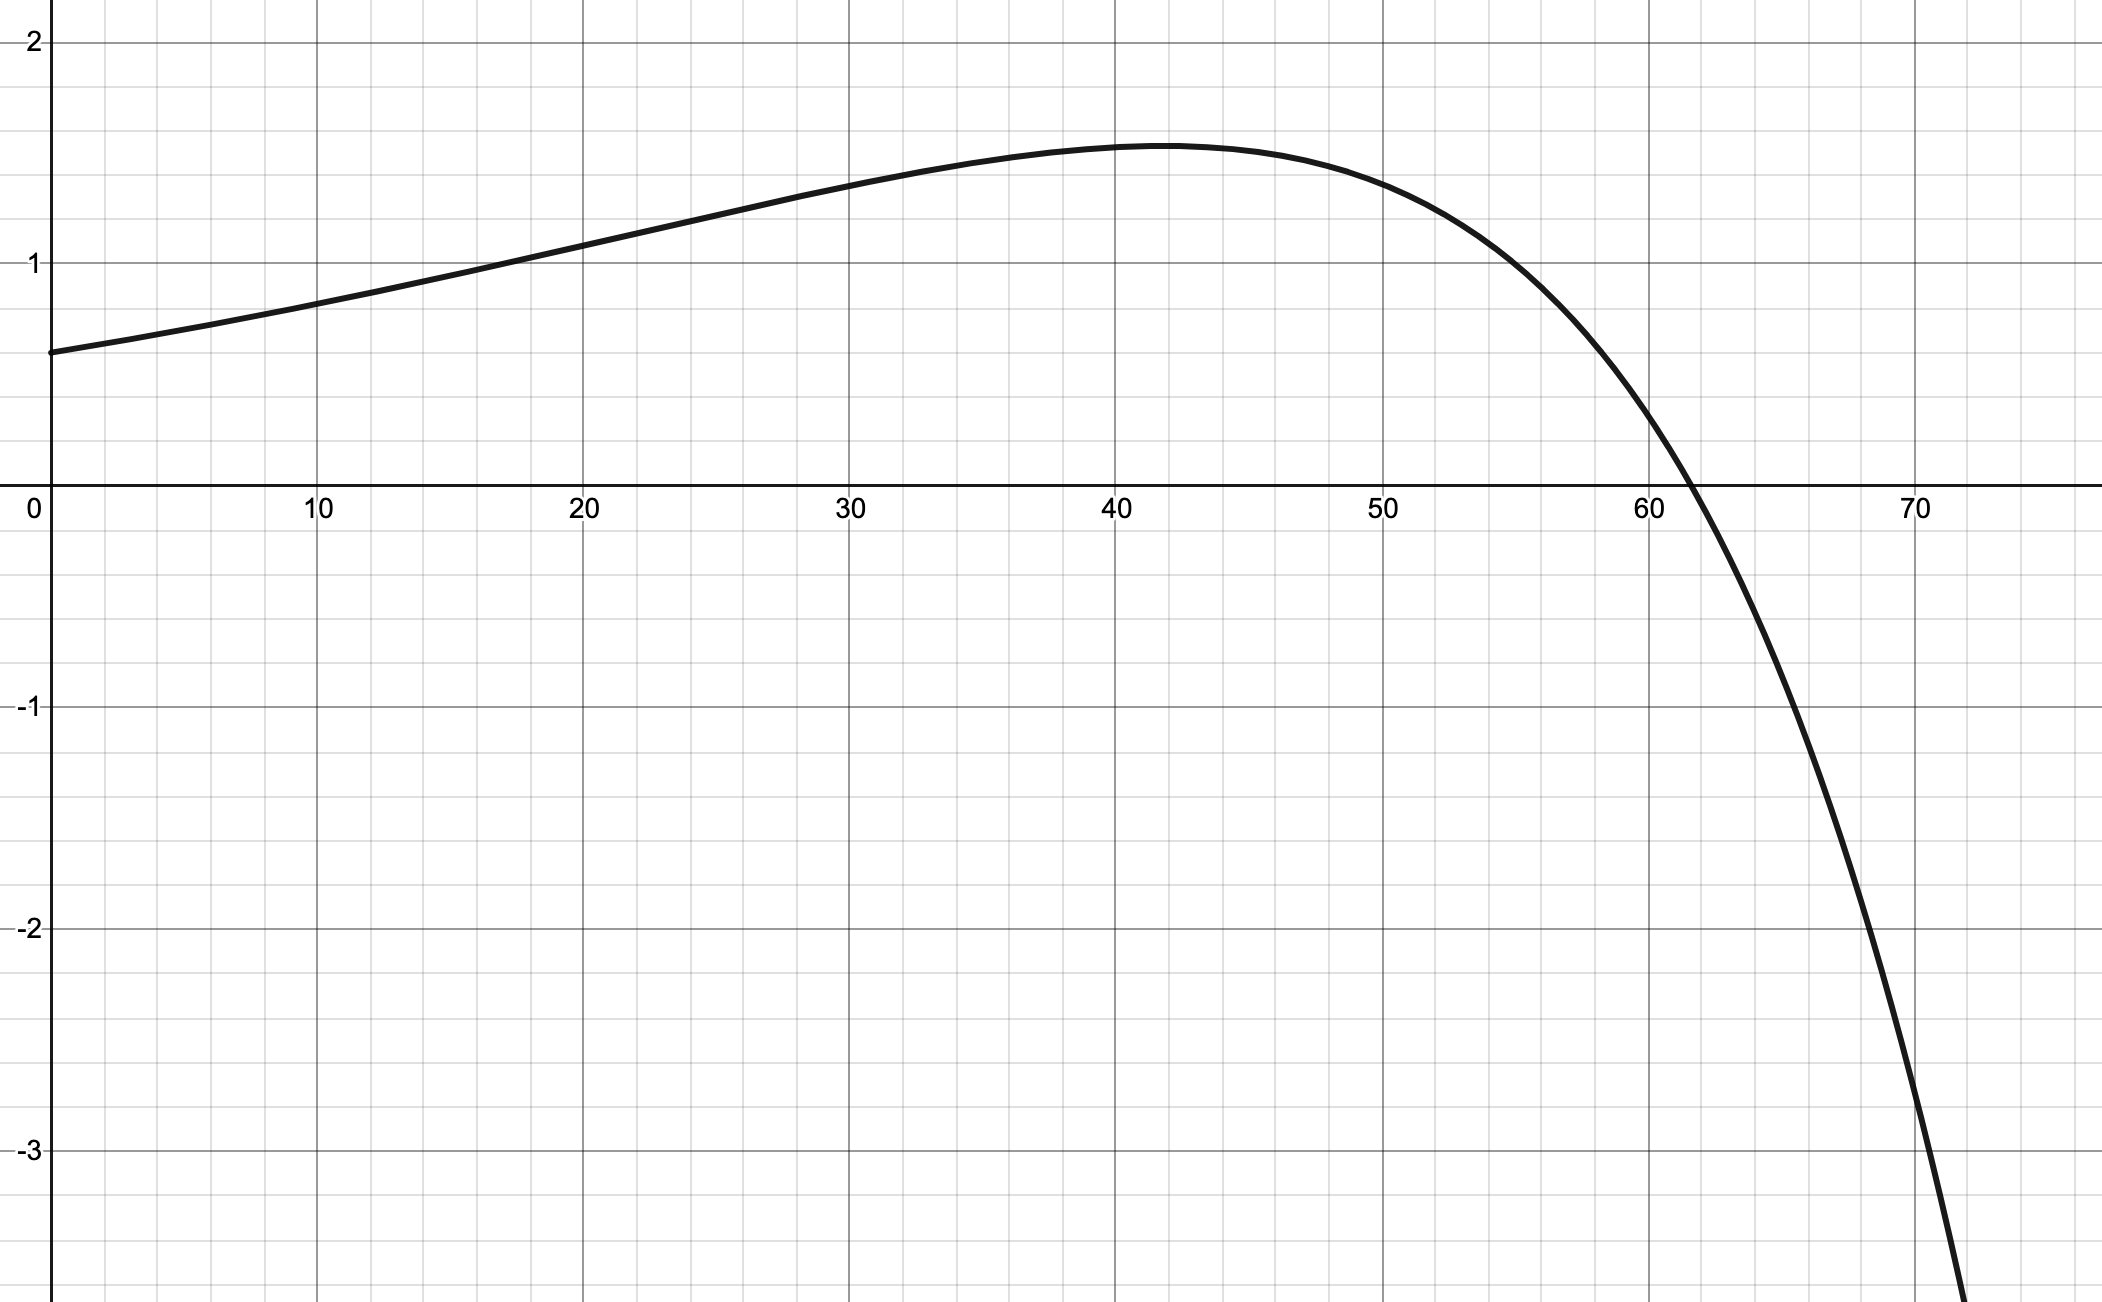
\includegraphics[scale=0.20]{images/netChange/birdPopulation1.png}
    \end{figure}
    %\vspace{2cm}
\item  What is the total number of birds after $10$ days? Use four decimal place.
    \begin{figure}[h!]
        \flushleft
        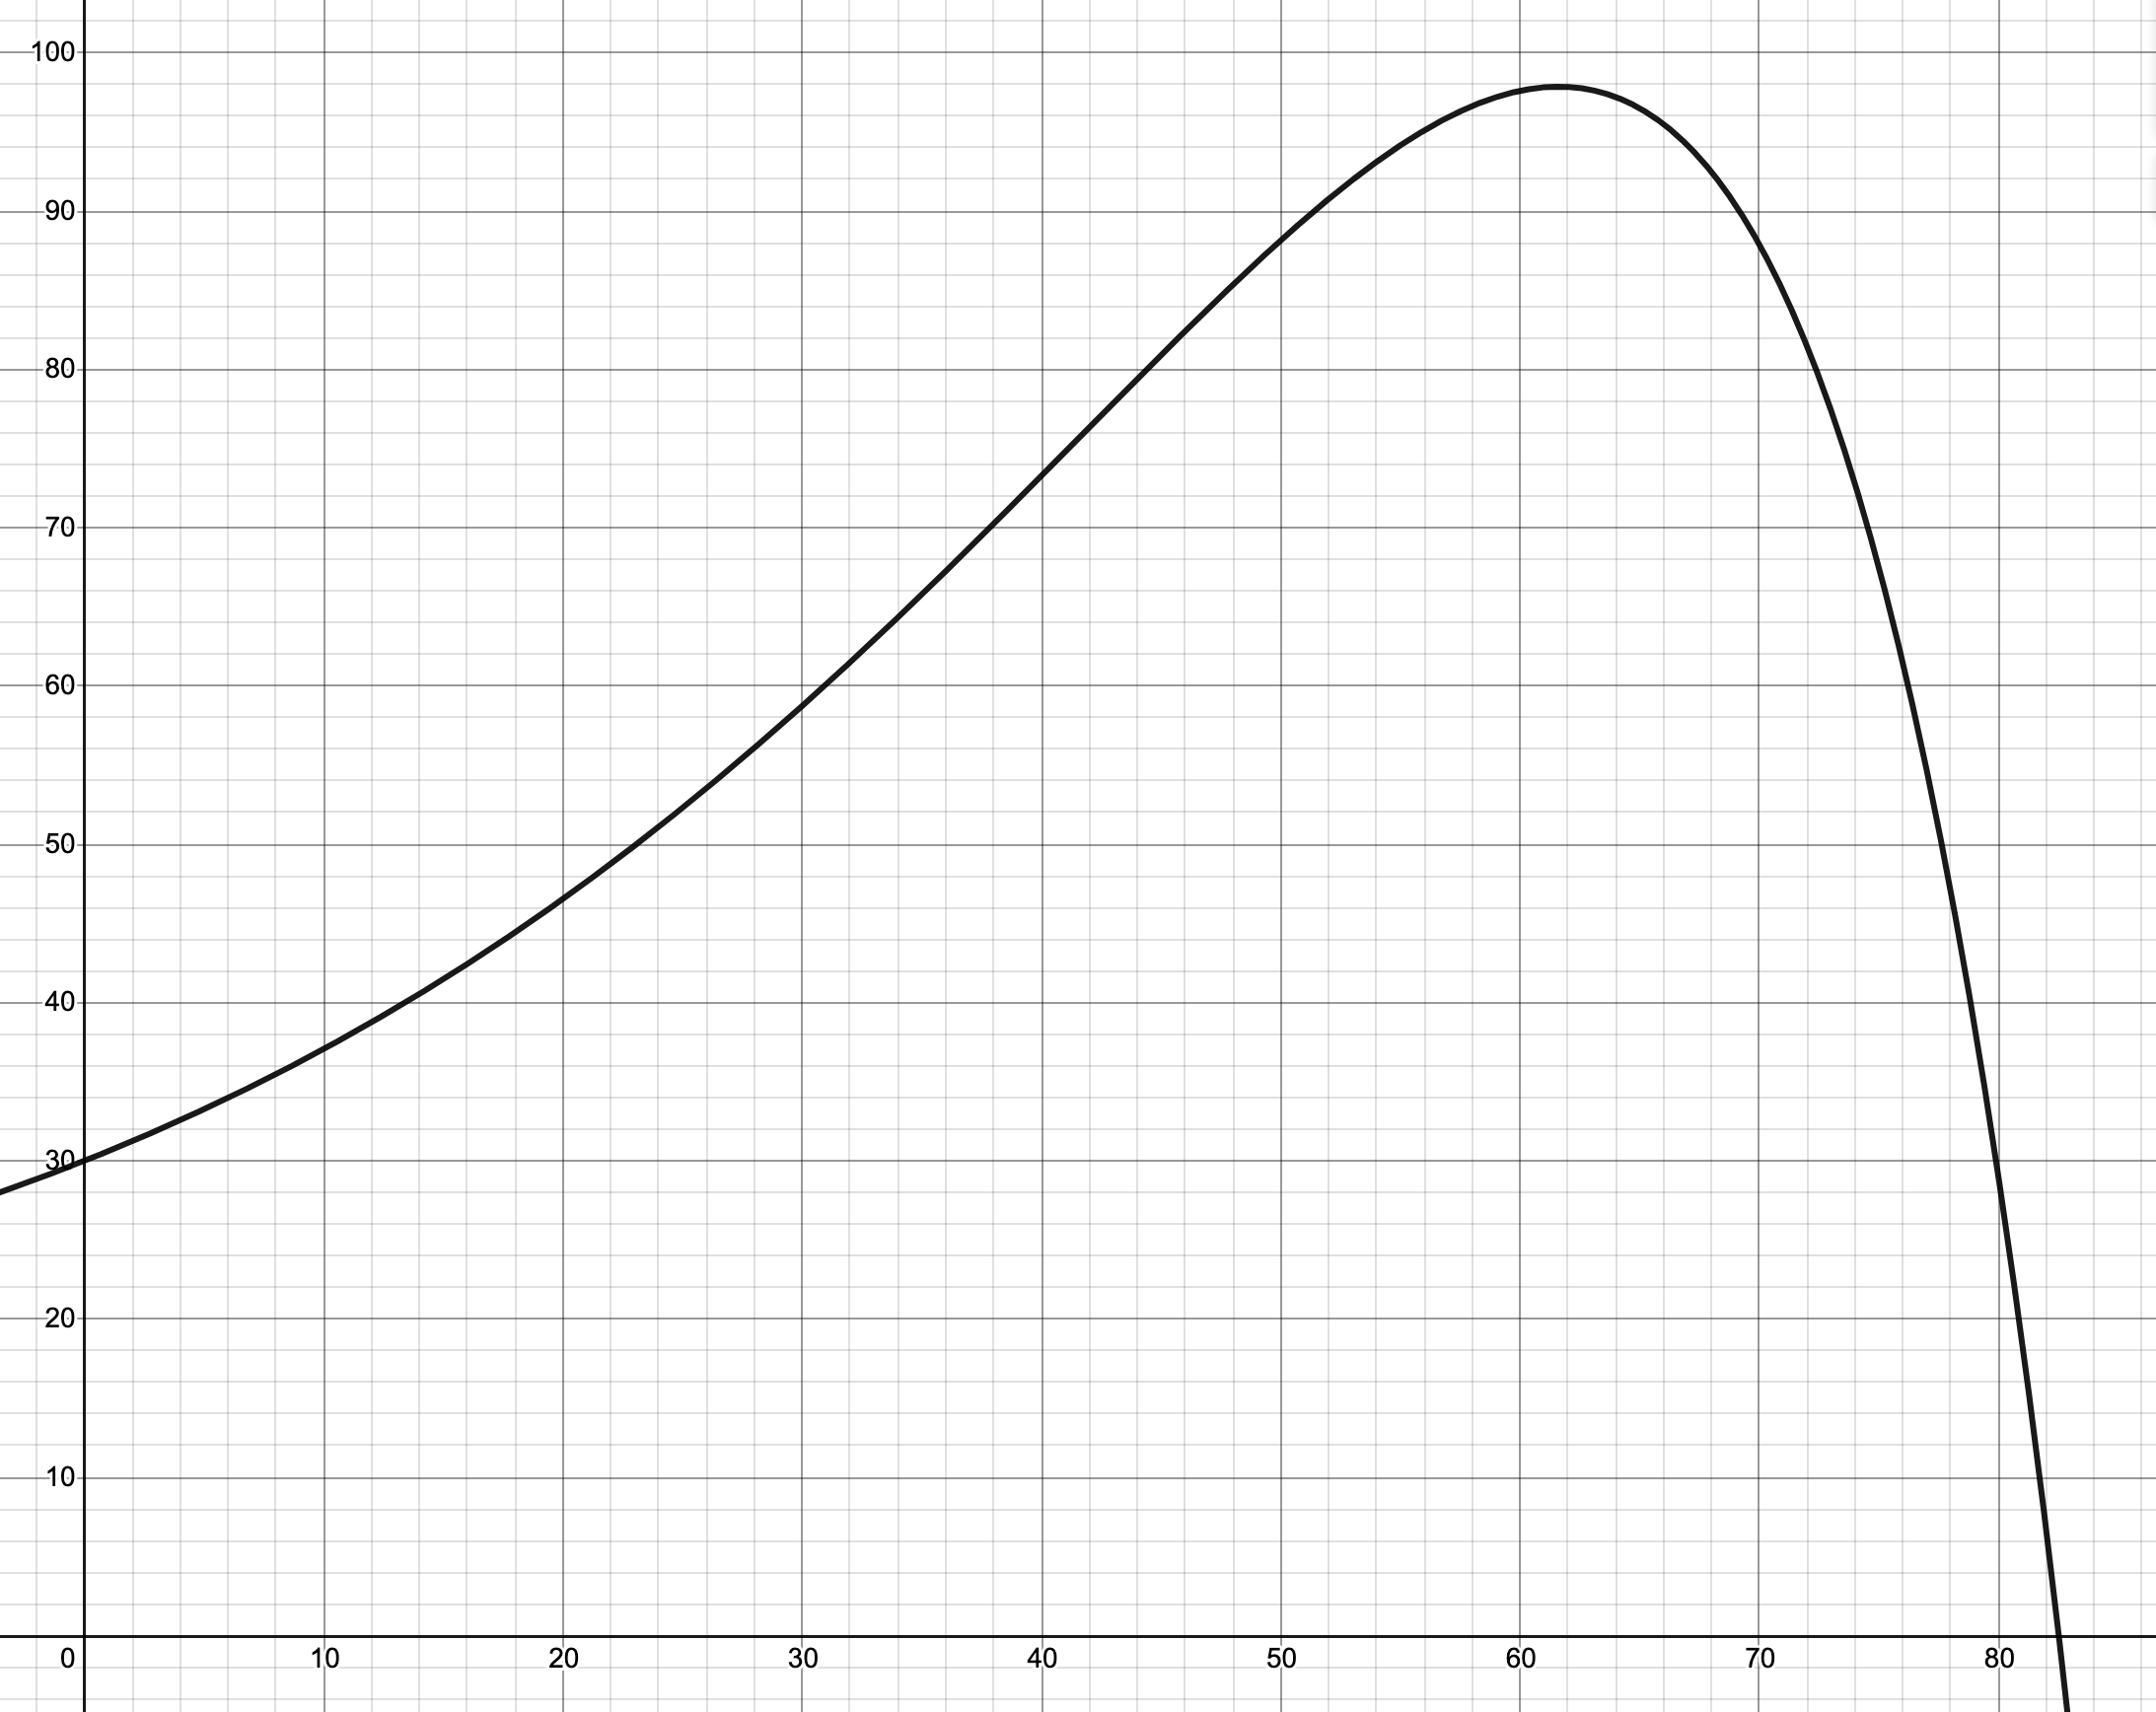
\includegraphics[scale=0.15]{images/netChange/birdPopulation2.png}
    \end{figure}
%\vspace*{\stretch{0.5}}
\newpage
\item During the first 20 days, what is the net change in total number of birds at the refuge ? 
\begin{figure}[h!]
        \flushleft
        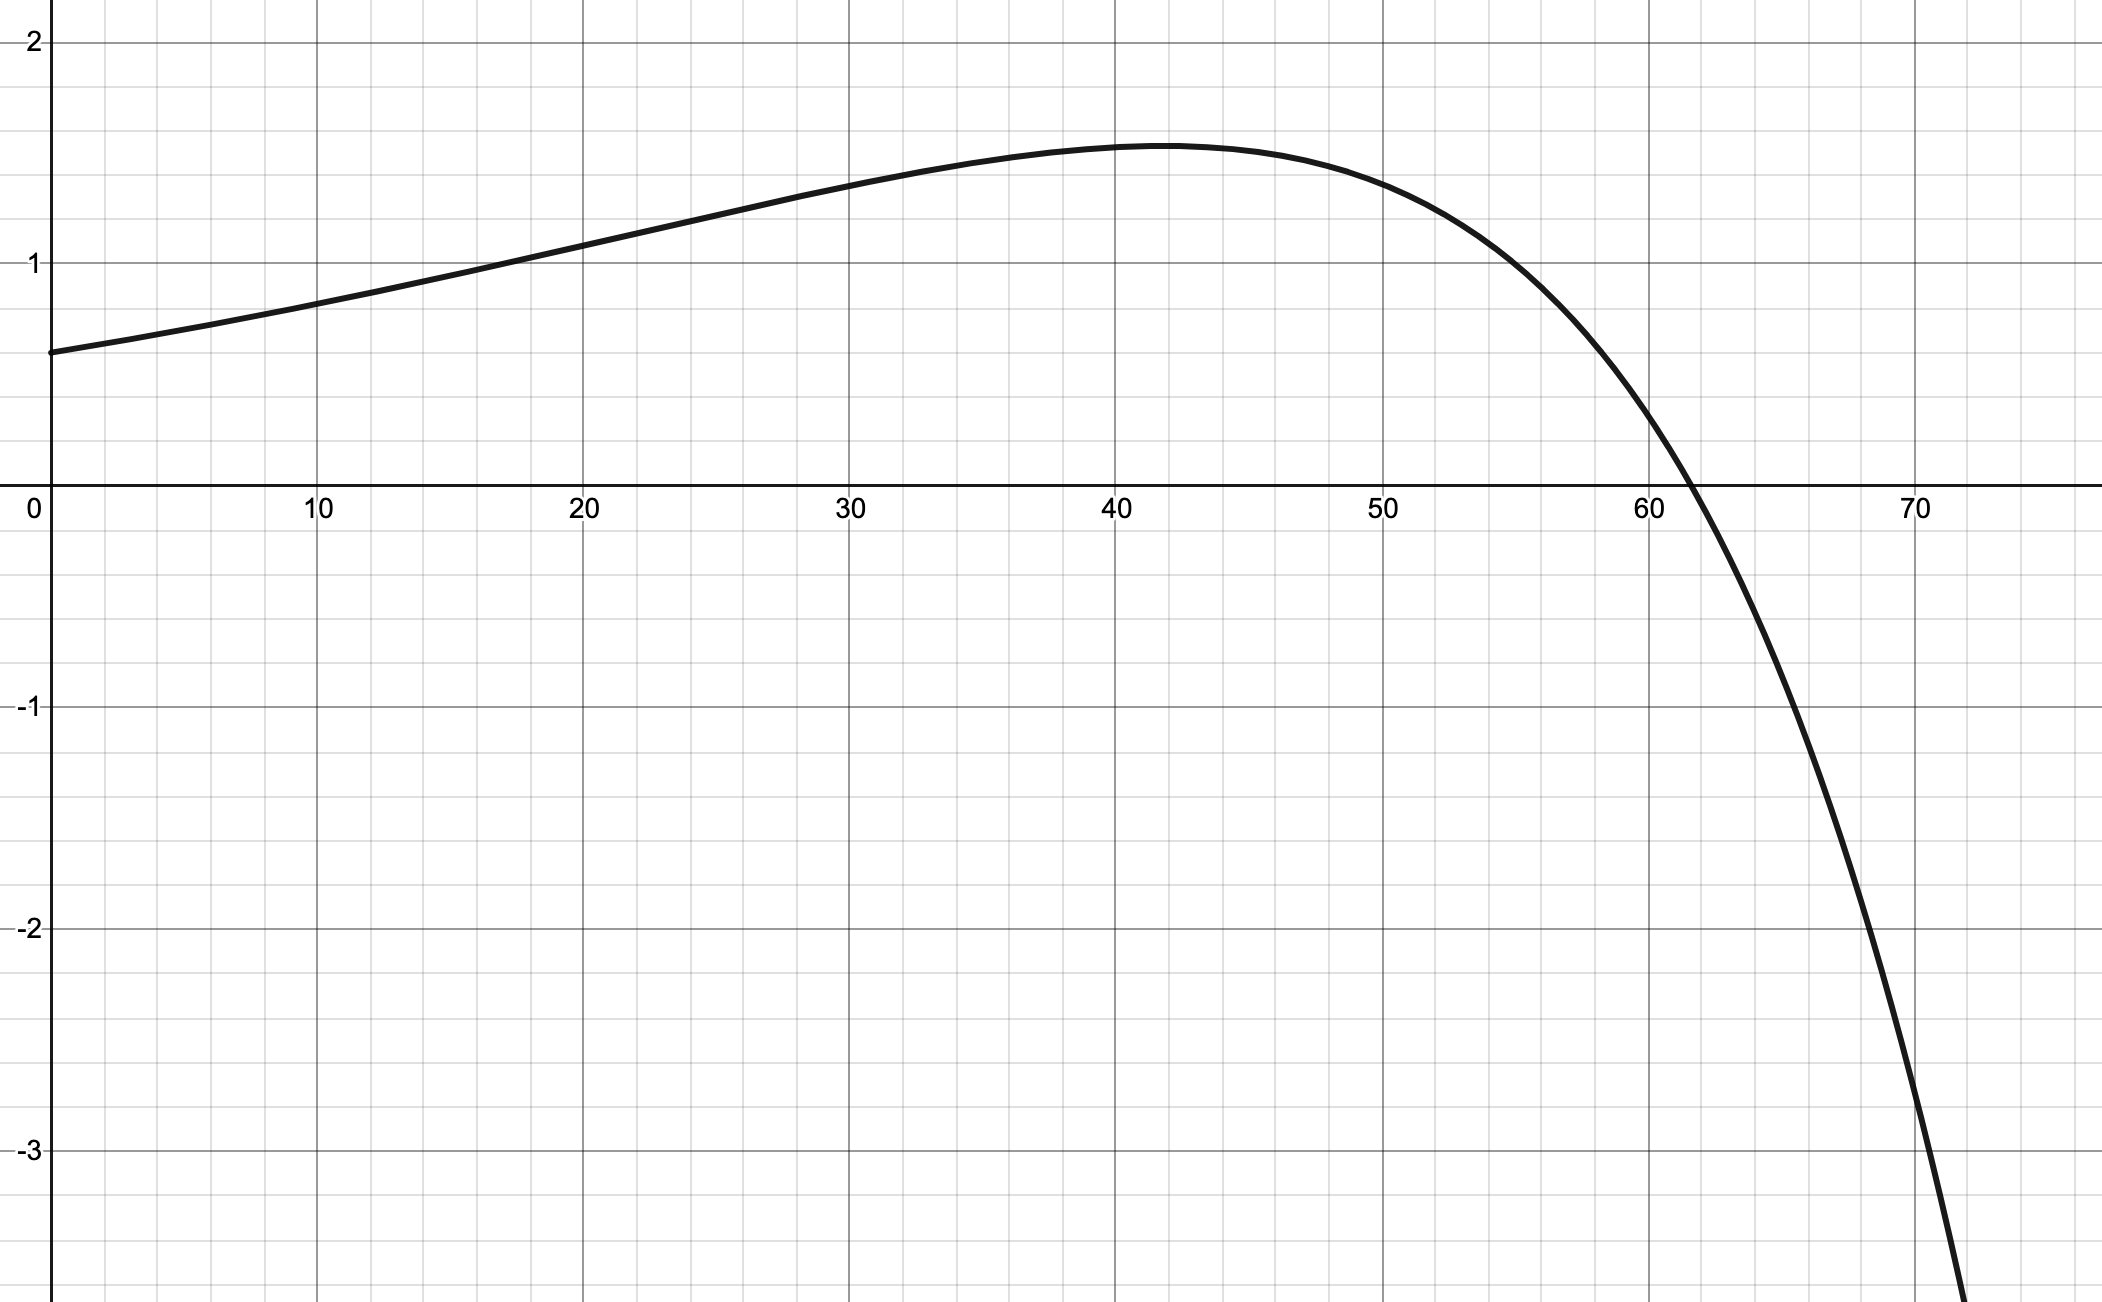
\includegraphics[scale=0.20]{images/netChange/birdPopulation1.png}
    \end{figure}
\vspace*{\stretch{1}}
\item What is the total number of birds after $20$ days? Use four decimal place.
\begin{figure}[h!]
        \flushleft
        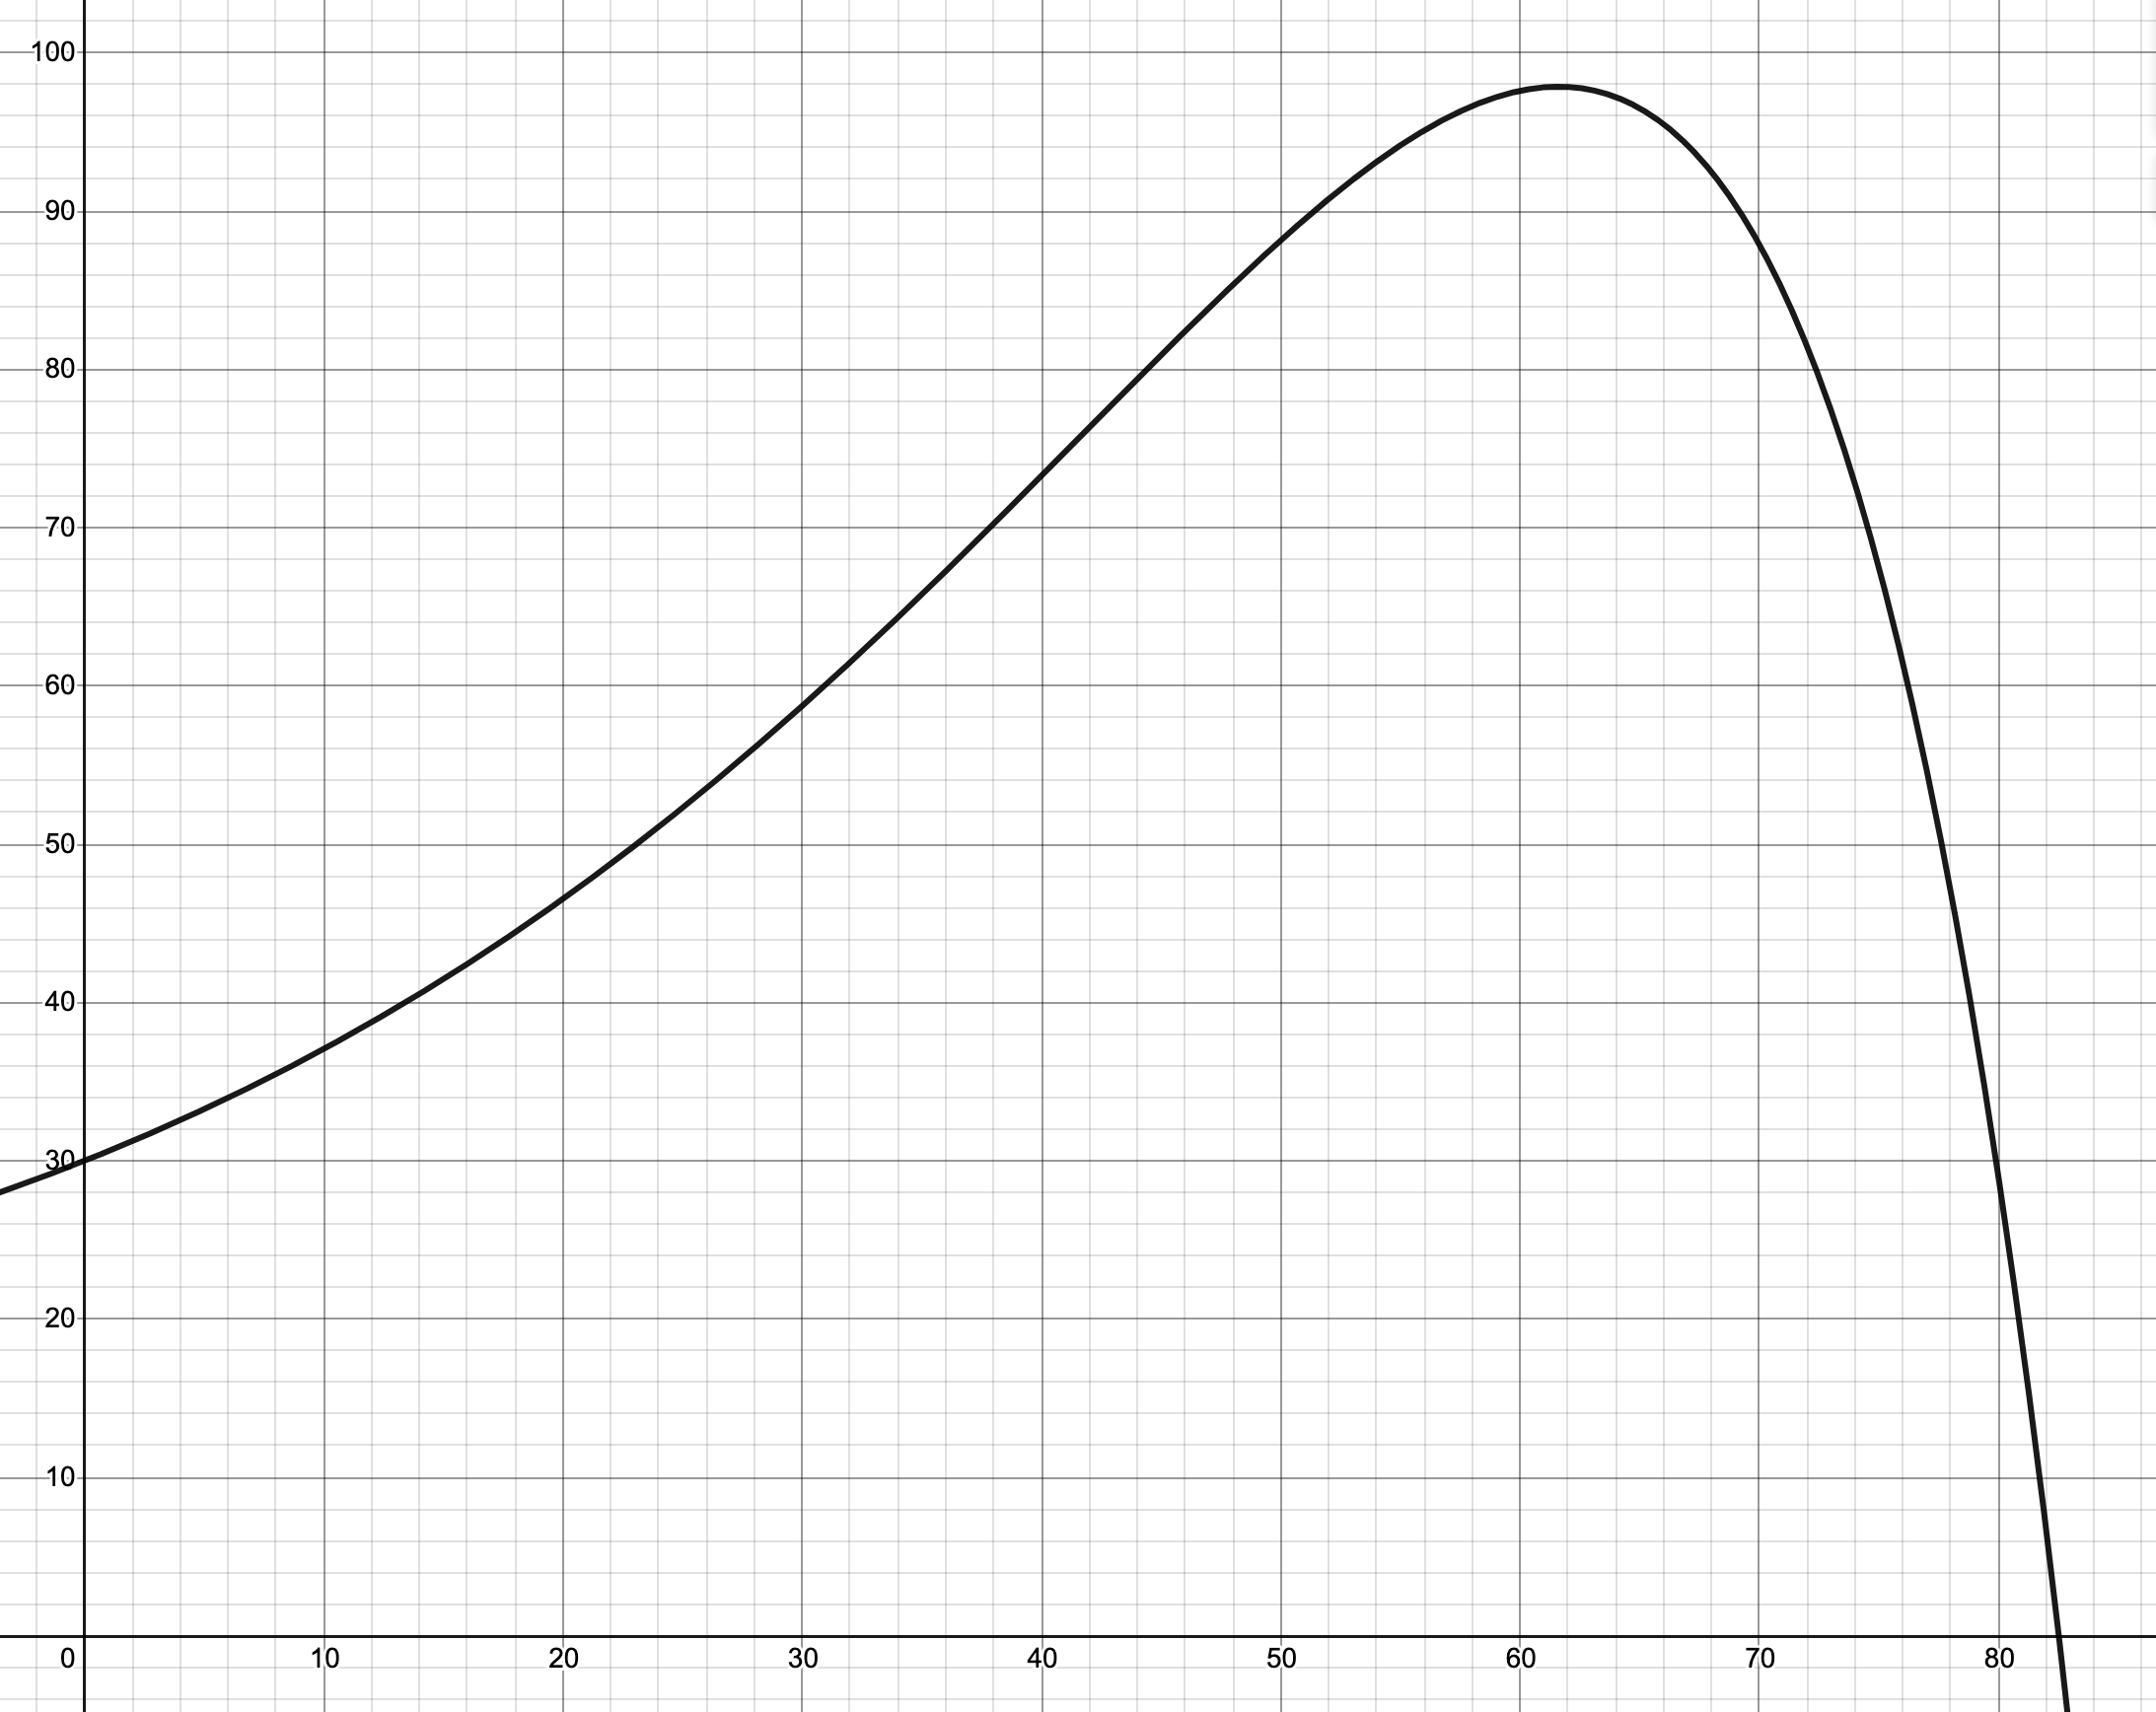
\includegraphics[scale=0.15]{images/netChange/birdPopulation2.png}
    \end{figure}
\vspace*{\stretch{0.5}}

\item Find the net change in the population size from time $t=10$ days to $t=20$ days.  Is the population increasing or decreasing over this time interval? By how many? Use one decimal place in your answer.
\begin{figure}[h!]
        \flushleft
        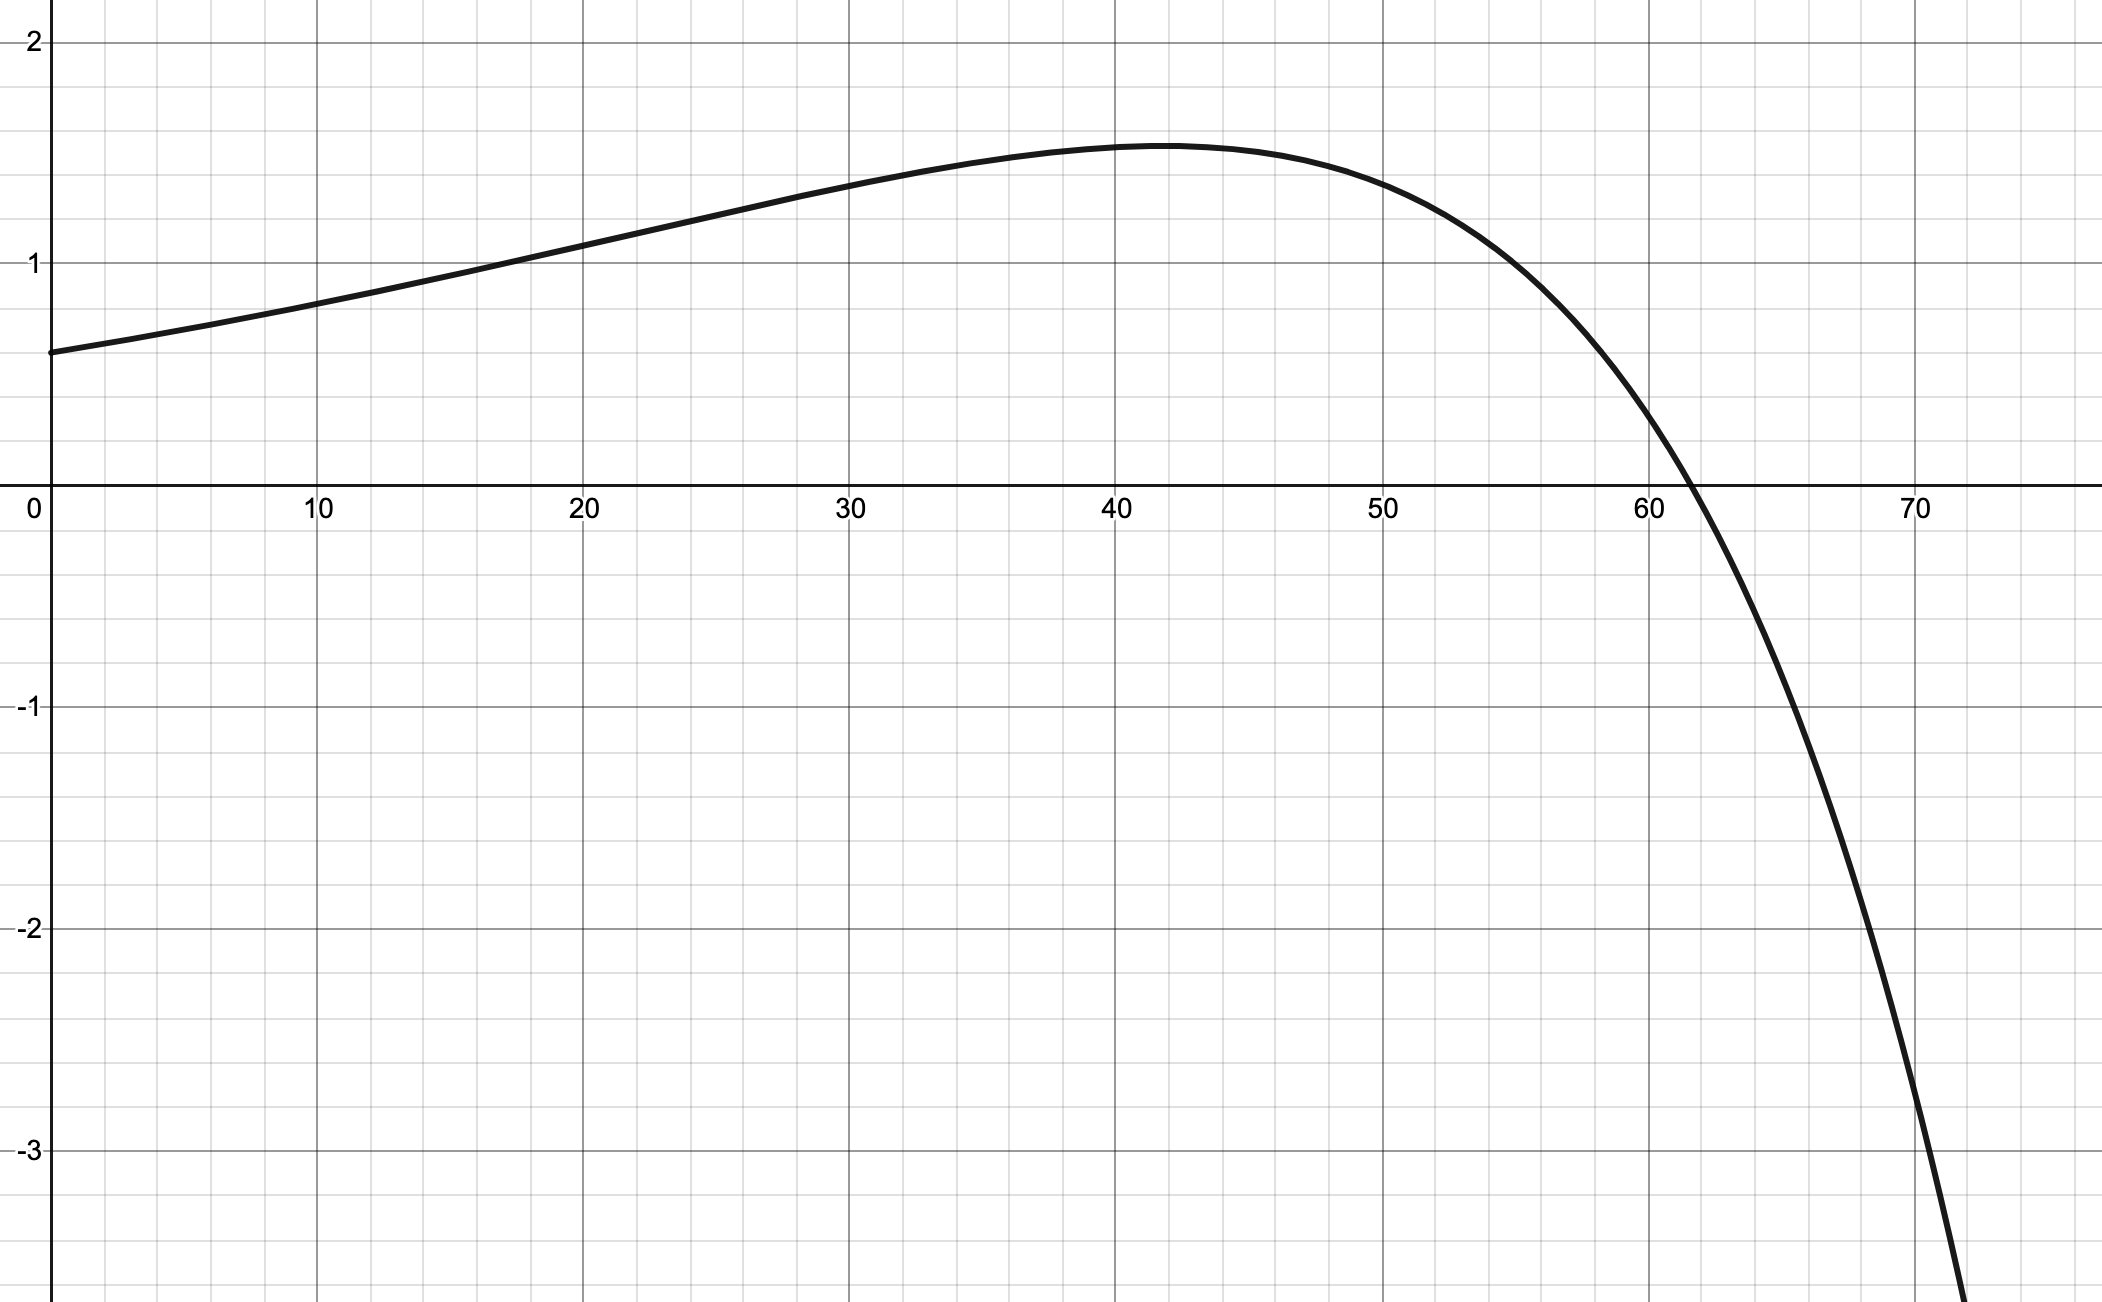
\includegraphics[scale=0.20]{images/netChange/birdPopulation1.png}
    \end{figure}
\vspace*{\stretch{0.5}}
\newpage
\item Find the net change in the population size from time $t=55$ days to $t=70$ days.  Is the population increasing or decreasing over this time interval?  Use one decimal place. 
\begin{figure}[h!]
        \flushleft
        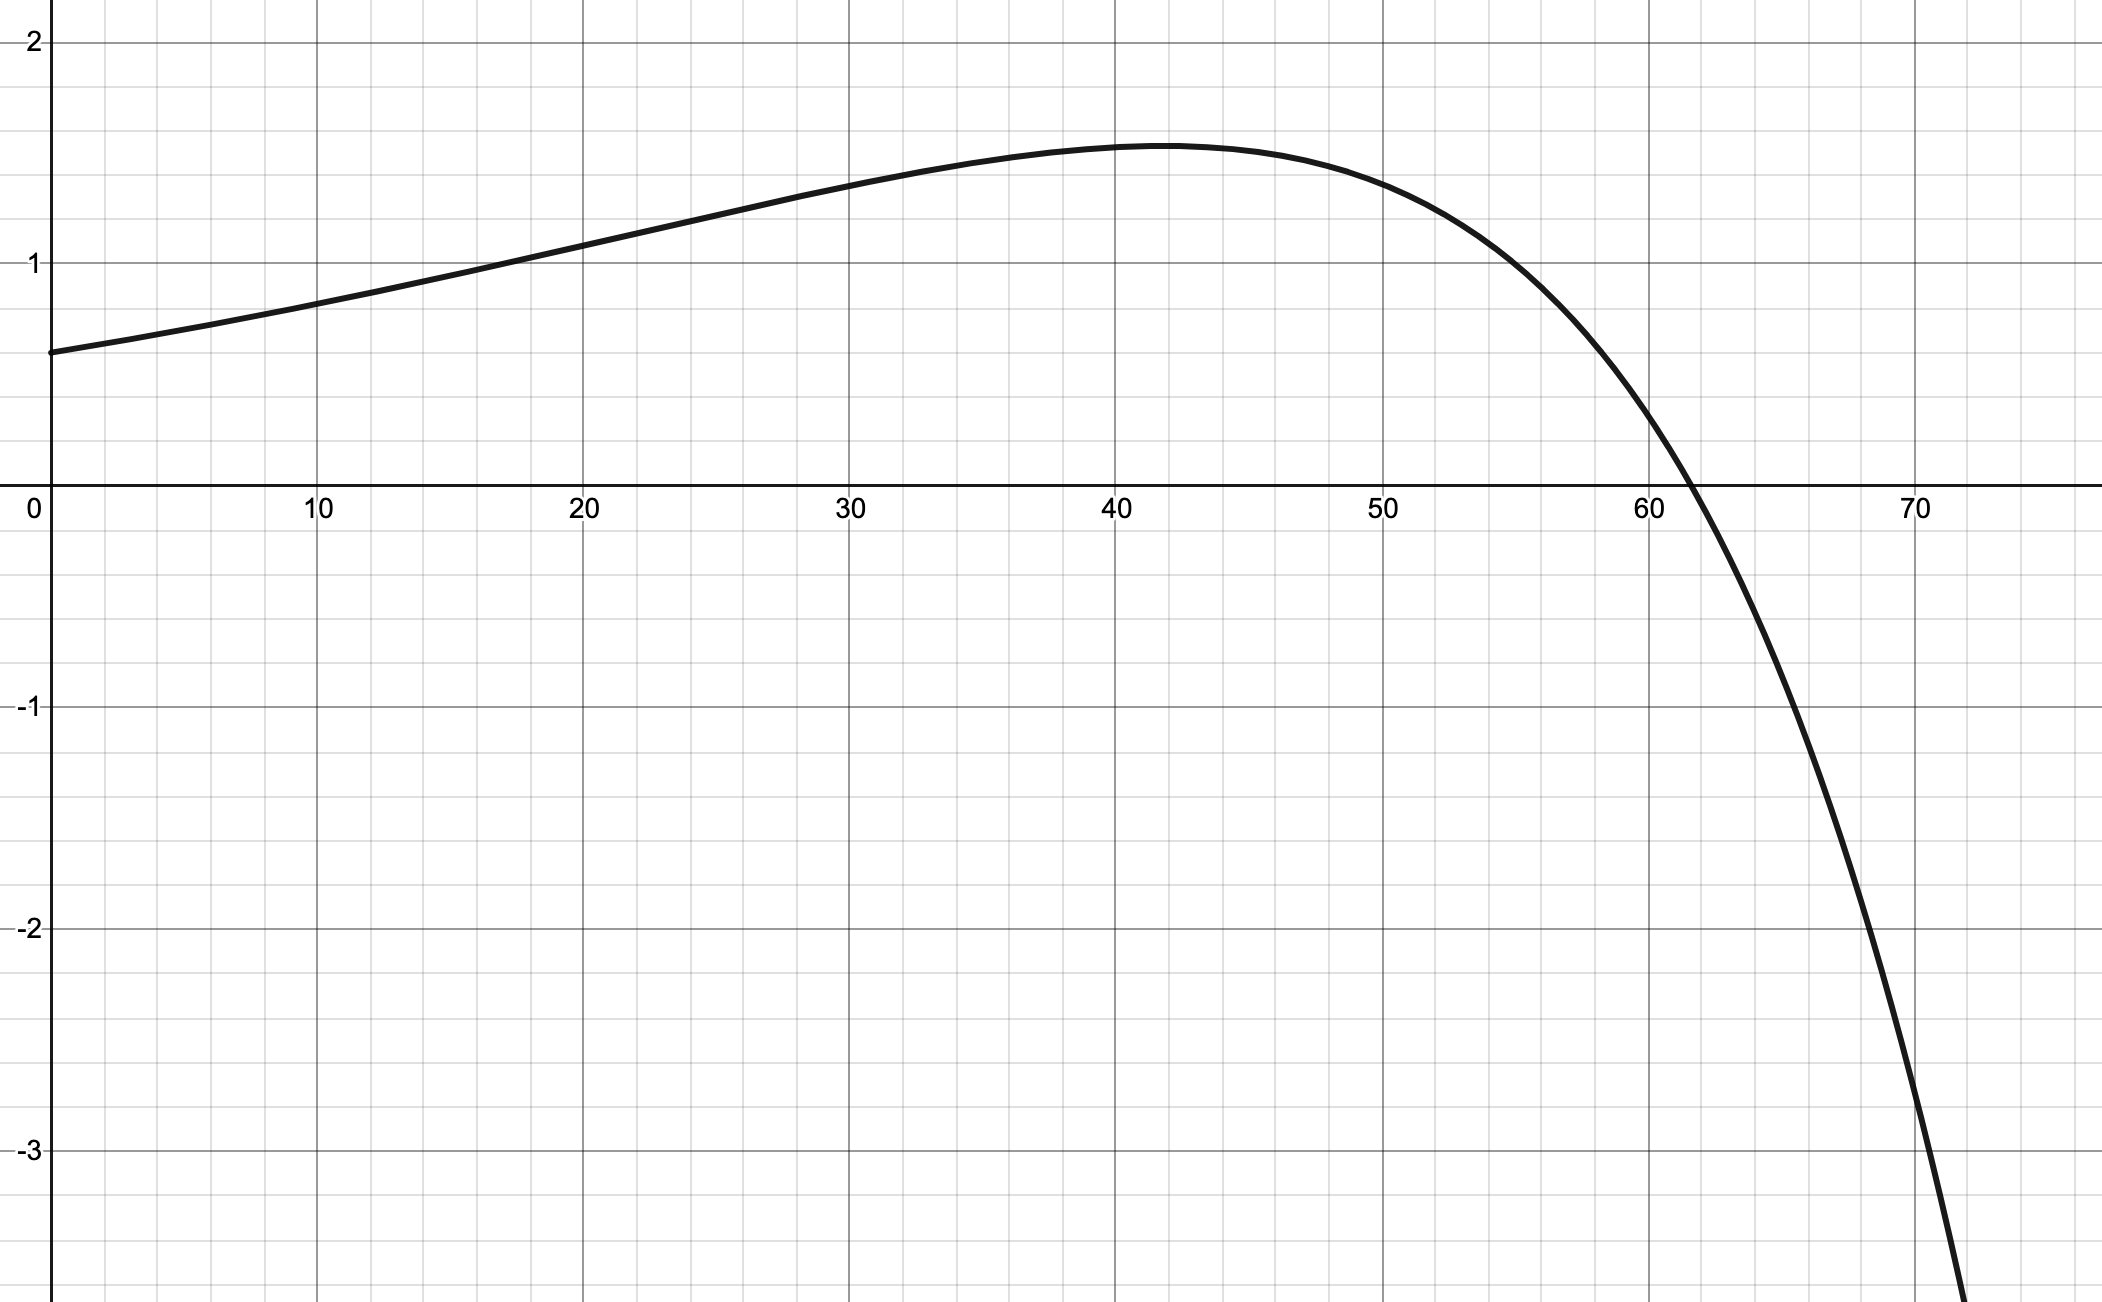
\includegraphics[scale=0.20]{images/netChange/birdPopulation1.png}
    \end{figure}
\vspace*{\stretch{1}}
\item Find the total number of birds after $70$ days.
\begin{figure}[h!]
        \flushleft
        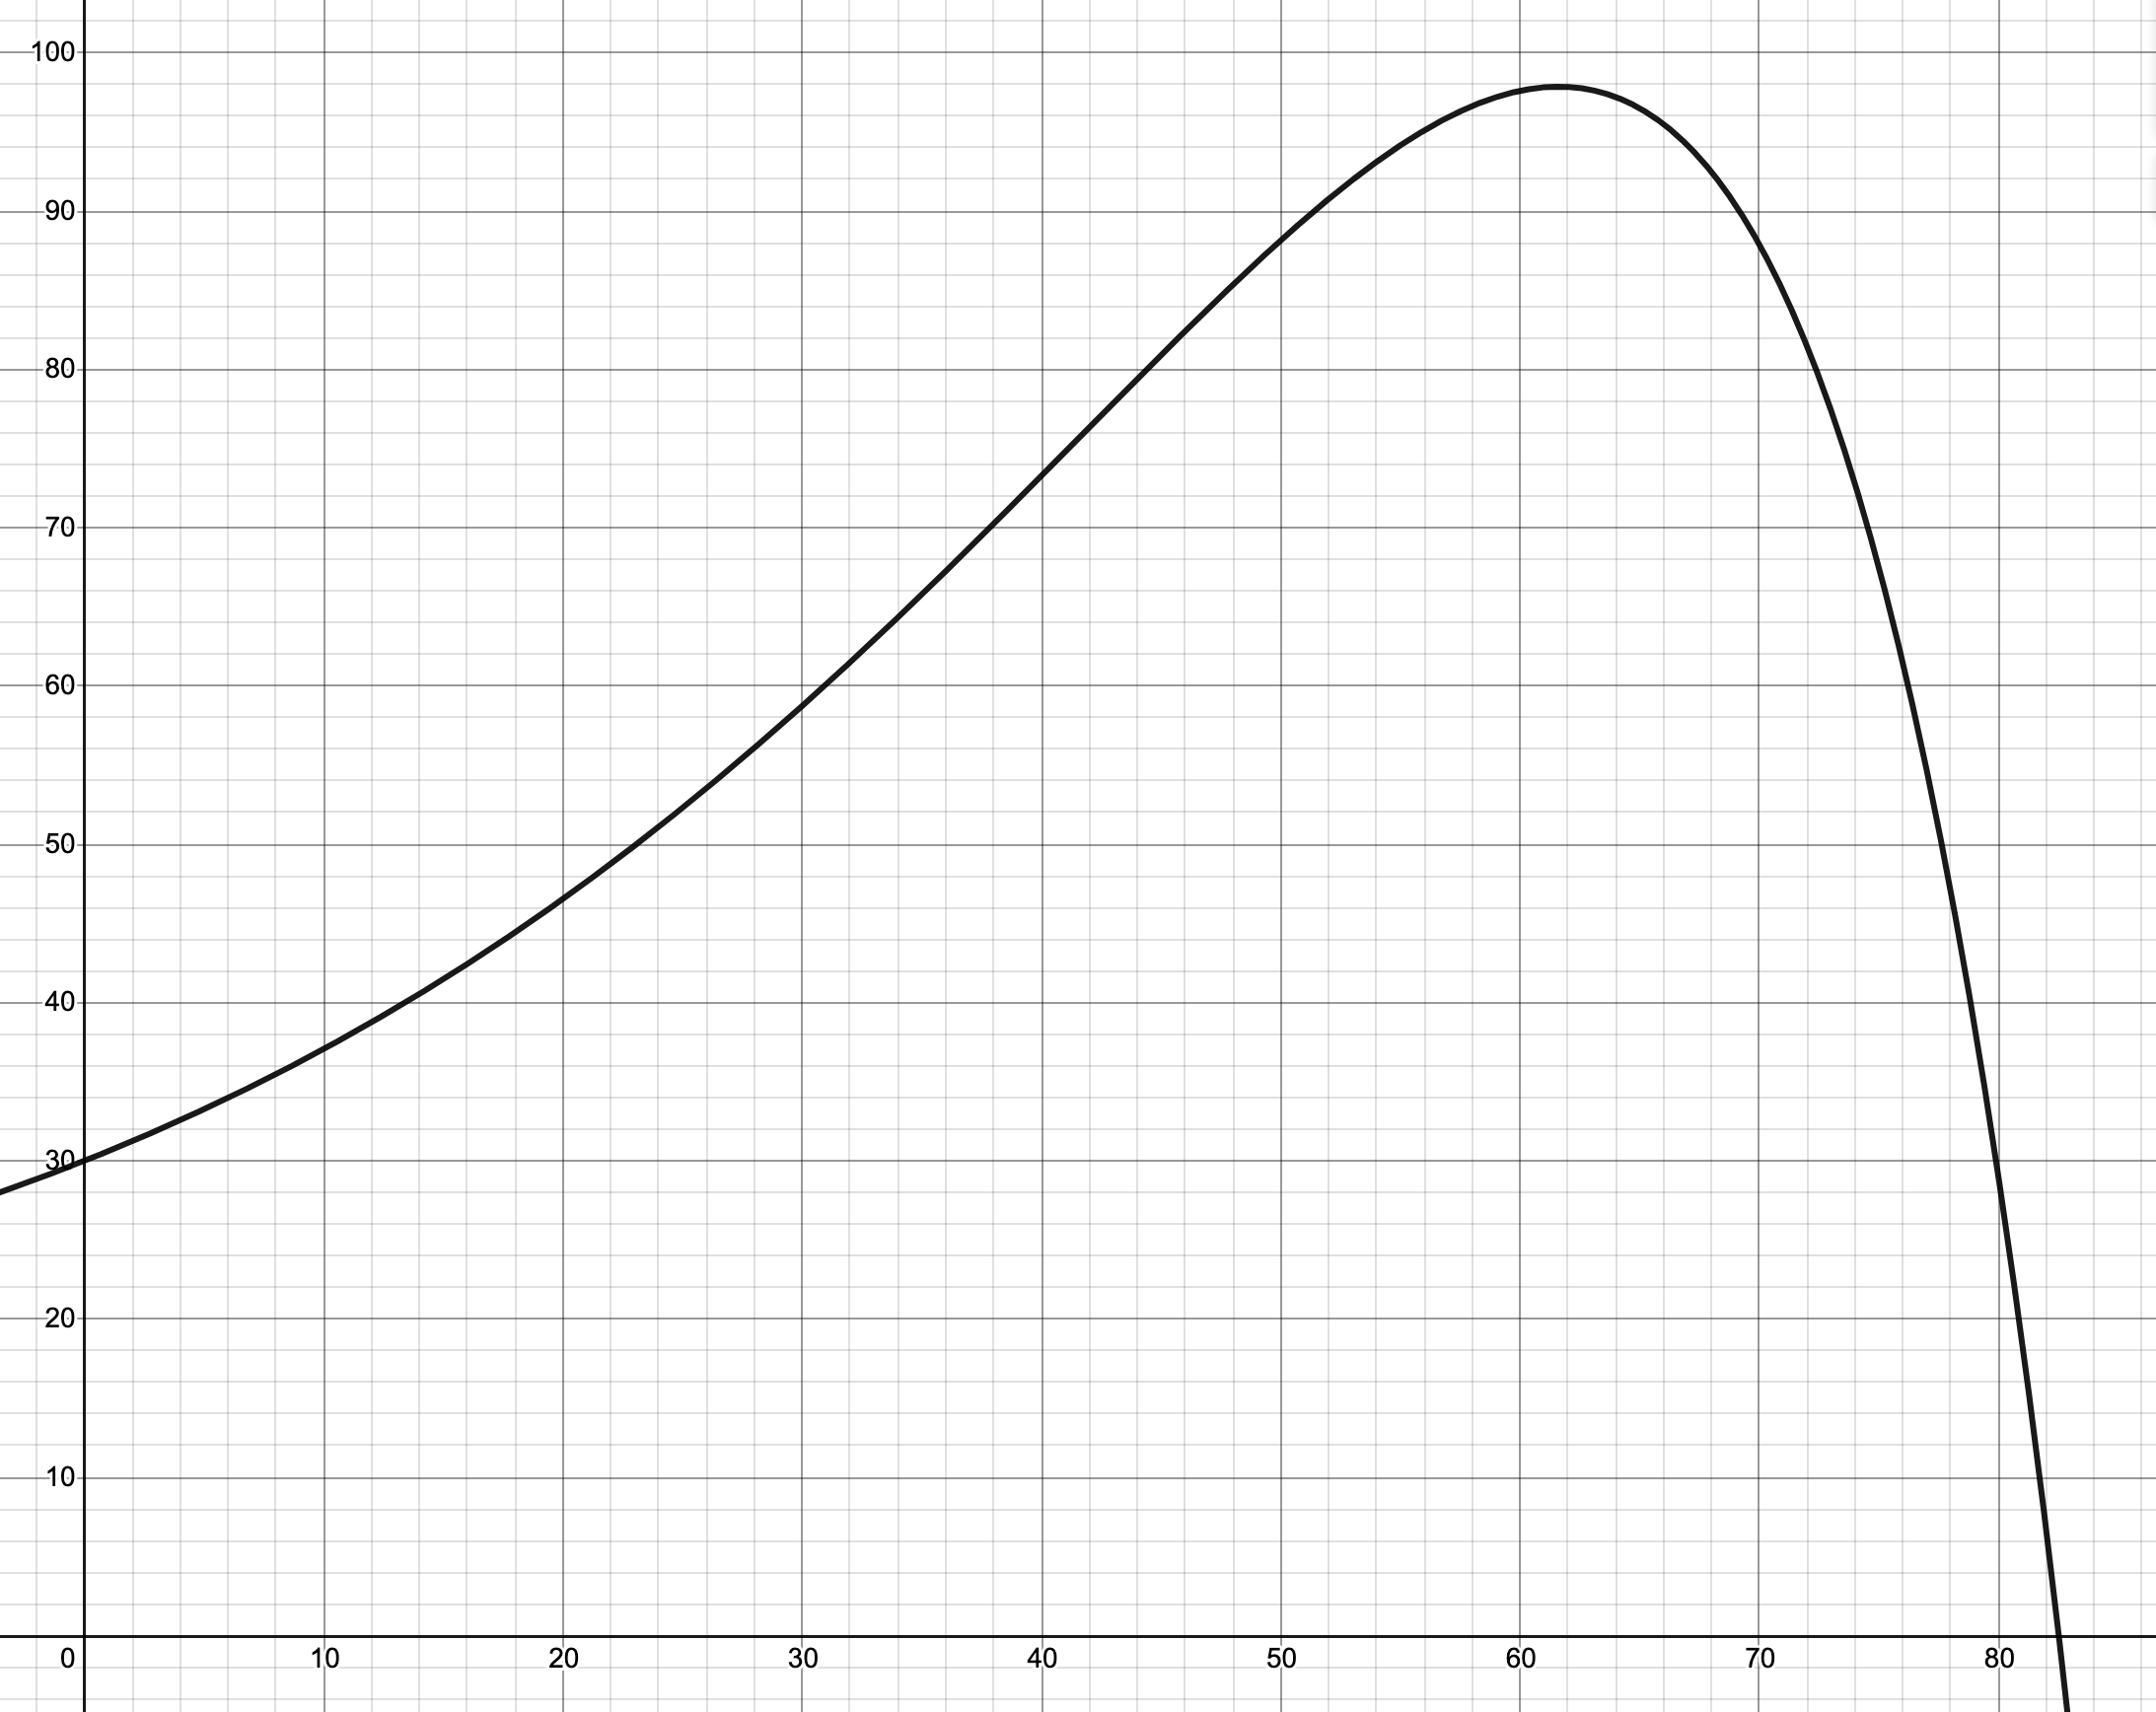
\includegraphics[scale=0.15]{images/netChange/birdPopulation2.png}
    \end{figure}
\vspace*{\stretch{0.5}}
\end{enumerate}
    %%short answer
    \begin{sol}
    \onehalfspacing{
    \begin{enumInline1}
    \item $P(t)=20e^{0.04t}-3.2e^{0.0625t}+C$
    \item $\int_{0}^{10} P'(x) dx\approx 7.0581$ hundreds of birds or about $706$ birds.
    \item $P(10)\approx 37.0581$ hundreds of birds or about $3,706$ birds.
    \item $\int_{0}^{20} P'(x) dx\approx 16.5417$ hundreds of birds or about $1,654$ birds.
    \item $P(20)\approx 46.5417$ hundreds of birds or about $4,654$ birds.
    \item $\int_{10}^{20} P'(x) dx\approx 9.4836$; We expect the population to \underline{increase} by approximately$\approx 9.4836$ hundreds or 9480 birds over the interval $t=10$ to $t=20$ days.
    \item $\int_{55}^{70} P'(x) dx \approx -6.2657$; We expect the population to \underline{decrease} (net change is negative or $\approx -6.2657$ hundreds of birds) by approximately $6.2657$ hundreds or 627 birds over the interval $t=55$ to $t=70$ days. 
    \item $P(70)\approx 87.8854$ hundreds of birds or about $8,789$.
    \end{enumInline1} }
    \end{sol}
    %%solution
    \begin{solL}
    ??
    
    \end{solL}
    
\end{example}

%%%%%%%%%%%%%%%%%%%%%%%%


%%%%%%%%%%%%%%%End Lesson%%%%%%%%%%%%%%%%%%
\Closesolutionfile{ans}
\Closesolutionfile{ansL}

%%%Short Answers to Examples%%%
%\newpage
\vspace*{\fill}

\subsection*{Short Answers to Examples}
%\vspace{-0.25cm}
%\begin{multicols}{2}
\input{ans21}
%\end{multicols}


